\documentclass[12pt]{article}

\usepackage{amsmath,amssymb,amsfonts,amsbsy}
%\usepackage{cite}
\usepackage{graphicx}
\usepackage[margin=20mm]{geometry}
\usepackage{wrapfig}
\usepackage[pagewise,displaymath]{lineno}
\usepackage{subfig}
\usepackage{epsfig}
\usepackage{authblk}
\usepackage[d]{esvect}
\usepackage{calc}
\usepackage[colorlinks=false,bookmarks=false,pageanchor=true]{hyperref}

\newcommand{\missET}{\vv{\not{\!\!E}}_T}
\newcommand{\abs}[1]{\lvert#1\rvert}

\begin{document}

\setcounter{section}{0}
\setcounter{subsection}{0}
\setcounter{equation}{0}
\setcounter{figure}{0}
\setcounter{footnote}{0}
\setcounter{table}{0}


\title{Measurement of Vector Boson Asymmetry in Transveresely Polarized $pp$
Collisions at RHIC}

\author{Elke Ashchenauer}
\author{Salvatore Fazio\thanks{fazio@bnl.gov}}
\author{Dmitri Smirnov\thanks{dsmirnov@bnl.gov}}

\affil{Physics Department, Brookhaven National Lab}

\date{\today\\[1em]Version 2}

\maketitle

\newpage

\tableofcontents 

\newpage

\section{Introduction}

In this study we propose to measure the asymmetry of the vector bosons produced
in transversely polarized proton collisions at STAR. First, we focus on the $W$
bosons decayed into a lepton pair ($W^\pm \to e^\pm \nu_e$). However, most of the
developed formulae can be used in the measurement of $Z$ boson asymmetry, and
we will consider this case later. From the measured asymmetry it is possible to
verify theoretical expectations about the sign change of the Sivers function in
Drell-Yan and SIDIS interactions:
%
\begin{equation}
f^\text{SIDIS}_{q/h^\uparrow} (x, k_\perp) = - f^\text{DY}_{q/h^\uparrow} (x, k_\perp).
\end{equation}

The single spin asymmetry (SSA) $A_N$ for the $W$ bosons and the lepton $l$
from the $W$ decay has been derived in \cite{Kang:2009bp, zpaper}. It is
parametrized based on the fits of SIDIS data and given as a function of
direction and transverse momentum. For the case of $W$ we have:
%
\begin{equation}
A^W_N = A^W_N(y_W, \phi_W, q_T) \equiv A_N(y, \phi, p_T) = A_N(\Omega, p_T),
\label{eq:asym_wboson}
\end{equation}
%
where $\Omega = \{y, \phi\}$ is simply used as a shorthand for the direction of
the particle in the lab frame. Similarly, for the lepton the expectated
asymmetry depends on the direction of the lepton and its transverse momentum:
%
\begin{equation}
A^l_N = A^l_N(\eta_l, \phi_l, p_T) \equiv A_N(y, \phi, p_T) = A_N(\Omega, p_T)
\label{eq:asym_lepton}
\end{equation}



\section{Experimental Viewpoint}

For the SSA measurements we are interested in the proton interactions
$p^{\uparrow/\downarrow} p \to W^\pm \to e^\pm \nu_e$ in which the spin direction of one
of the protons is irrelevant, \textit{i.e} unpolarized protons. In the
experiment we can separately measure full and differential cross sections for
spin-up ($\sigma_\uparrow$), spin-down ($\sigma_\downarrow$), and unpolarized
($\sigma_0$) interactions which are related as:
%
\begin{align}
\sigma_\uparrow   &= \sigma_0 (1 + A_N ), \\
\sigma_\downarrow &= \sigma_0 (1 - A_N ).
\end{align}
%
In the following we assume that the polarization vector does not significantly
deviate from the vertical direction given by the normal unit vector $\vec n$
along the vertical $y$ axis so, the notation is $P \equiv \vec{P} \cdot
\vec{n}$. We also assume the same magnitude of the polarization vector for
spin-up and spin-down bunches, \textit{i.e.} $P = P_\uparrow = P_\downarrow$.
For unpolarized cross section $\sigma_0 \equiv (\sigma_\uparrow +
\sigma_\downarrow)/2$ the asymmetry $A_N$ is expressed as:
%
\begin{align}
\label{eq_anapower}
A_N &= \frac{\sigma_\uparrow - \sigma_\downarrow}{\sigma_\uparrow +
   \sigma_\downarrow}.
\end{align}

The number of recorded events in which the particle is produced with momentum
$p_T$ at angle $\Omega$ is:
%
\begin{align}
\frac{dN_{\uparrow/\downarrow}}{d\Omega dp_T}(\Omega, p_T) &=
   {\cal L}_{\uparrow/\downarrow} \frac{d\sigma_0}{d\Omega dp_T}(\Omega, p_T)
   \varepsilon(\Omega, p_T) \big( 1 \pm A_N(\Omega, p_T) P \big),
\label{eq:yield_diff}
\end{align}
%
where detection efficiency $\varepsilon$ does not depend on the spin direction
of the interacting proton. In fact, individual events can be tagged by the
nominal spin of colliding protons. We thus can bin all collected data  in four
bins $N_{\uparrow\uparrow}$, $N_{\uparrow\downarrow}$,
$N_{\downarrow\uparrow}$, and $N_{\downarrow\downarrow}$. For the SSA
measurement the polarization of one of the beams is ignored by combining the
yields with opposite spins, \textit{e.g.}
%
\begin{align}
N_{\uparrow}   \equiv N_{\uparrow0}   &= N_{\uparrow\uparrow}   + R_{\frac{0\uparrow}{0\downarrow}} N_{\uparrow\downarrow},\\
N_{\downarrow} \equiv N_{\downarrow0} &= N_{\downarrow\uparrow} + R_{\frac{0\uparrow}{0\downarrow}} N_{\downarrow\downarrow},
\end{align}
%
where re-weighting factor $R_{\frac{0\uparrow}{0\downarrow}}$ addresses a
possible relative difference in the spin-up and spin-down intensities of the
other beam. Studies have shown that $R_{\frac{0\uparrow}{0\downarrow}} \approx
1$ with good precision.

We bin our data sample in three observable variables $\{y, \phi, p_T\}$ with
center and width of the $i$-th bin being $\{y_i, \phi_i, p_{T,i}\}$ and
$\{\Delta y_i, \Delta\phi_i, \Delta p_{T,i}\} \equiv \{\Delta\Omega_i\{y_i,
\Delta\phi_i\}, \Delta p_{T,i}\} \equiv \Delta_i$ respectively. The number of
events in each bin, $N_i$, is calculated by integrating both sides
of~\eqref{eq:yield_diff} within the bin:
%
\begin{align}
N_{\uparrow/\downarrow, i} =
   \int\limits_{\Delta_i} \frac{dN_{\uparrow/\downarrow}}{d\Omega dp_T} d\Omega dp_T.
\end{align}
%
In that bin we assume the average value:
%
\begin{align}
A_{N,i} = \frac{1}{\Delta_i} \int\limits_{\Delta_i} A_N d\Omega dp_T,
\end{align}
%
and similarly for the cross section ($\sigma_{0,i}$) and efficiency
($\varepsilon_i$). Finally, for the yields in each bin we can write:
%
\begin{align}
N_{\uparrow/\downarrow, i} = {\cal L}_{\uparrow/\downarrow} \sigma_{0,i}
\varepsilon_i \Delta\Omega_i \Delta p_{T,i} \left( 1 \pm A_{N,i}(\Omega, p_T) P \right)
\label{eq:yield}
\end{align}

The spacial distributions of the physical asymmetry and the cross sections are
the same for the spin-up and spin-down interactions with respect to the spin
direction. We can use this fact to easily get rid of the  quantities of no
interest in \eqref{eq:yield}. This is achieved by constructing geometric
means $\sqrt{N_\uparrow(\phi_i)N_\downarrow(\phi_i+\pi)}$ and
$\sqrt{N_\uparrow(\phi_i+\pi)N_\downarrow(\phi_i)}$ of the yields
%
%
\begin{align}
N_\uparrow(\phi_i)       &= {\cal L_\uparrow}
   \sigma_{0}(\phi_i) \varepsilon(\phi_i)    \Delta\Omega_i \Delta p_T \left( 1 + A_{N}(\phi_i) P \right) \\
%
N_\uparrow(\phi_i+\pi)       &= {\cal L_\uparrow}
   \sigma_{0}(\phi_i+\pi) \varepsilon(\phi_i+\pi)    \Delta\Omega_i \Delta p_T \left( 1 + A_{N}(\phi_i+\pi) P \right)
\end{align}
%
%
\begin{align}
N_\downarrow(\phi_i+\pi) &= {\cal L_\downarrow}
   \sigma_{0}(\phi_i+\pi) \varepsilon(\phi_i+\pi) \Delta\Omega_i \Delta p_T \left( 1 - A_{N}(\phi_i+\pi) P \right) \\
%
N_\downarrow(\phi_i) &= {\cal L_\downarrow}
   \sigma_{0}(\phi_i) \varepsilon(\phi_i) \Delta\Omega_i \Delta p_T \left( 1 - A_{N}(\phi_i) P \right)
\end{align}
%
%
Using the relations for the asymmetry and cross section $A_{N}(\phi_i+\pi) =
-A_{N}(\phi_i)$, $\sigma_0(\phi_i+\pi) = \sigma_0(\phi_i)$ we get for $A_N$


\begin{align}
A_{N, i} = \frac{1}{P} \frac{%
\sqrt{N_{\uparrow}(\phi_i)N_{\downarrow}(\phi_i+\pi)} -
\sqrt{N_{\uparrow}(\phi_i+\pi)N_{\downarrow}(\phi_i)}
}{%
\sqrt{N_{\uparrow}(\phi_i)N_{\downarrow}(\phi_i+\pi)} +
\sqrt{N_{\uparrow}(\phi_i+\pi)N_{\downarrow}(\phi_i)}
}
\label{eq:asym_sqrt}
\end{align}



\section{Correction for Background}

In this analysis an optimal set of cuts is applied to select signal enriched
events without significant loss in the final statistics. The final yields
include some fraction of background events $f_B$ which along with the signal
asymmetry contribute to the measured asymmetry $A_N$. In order to extract the
signal asymmetry we decompose $A_N$ as following:
%
\begin{equation}
A_N = f_\text{sig} A^\text{sig}_N + f_B A^B_N,
\label{eq:asym_bkg}
\end{equation}
%
with $f_\text{sig} = 1 - f_B$. The last term in \eqref{eq:asym_bkg} may include
contributions from various backgrounds which will be discussed later. The
background fractions and asymmetries have to be estimated in order to extract
the final asymmetry of the signal:
%
\begin{equation}
A^\text{sig}_N = \frac{A_N + f_B A^B_N}{1 - f_B}
\label{eq_bkg_corr}
\end{equation}



\section{Sivers Sign Change Extraction}

A binned likelihood method can be used to check the sensitivity of our data to
the sign of the Sivers function. A direct way of doing this is to compare the
measured asymmetry \eqref{eq:asym_sqrt} with background corrected expectations
from \eqref{eq:asym_bkg}. The signal asymmetry $A^\text{sig}_N$ in this case
directly comes from the model predictions~\eqref{eq:asym_wboson} or
\eqref{eq:asym_lepton}. The simplest likelihood function can be constructed as a
product of gaussian terms over all bins:
%
\begin{equation}
L = \prod\limits_i G(A_{N,i}, \sigma_{A_{N,i}}; A^\text{sig}_{N,i}).
\end{equation}
%
Alternatively, the Sivers sign can be extracted from the Poisson probabilities
of measured given the expected yields.
%
\begin{equation}
L = \prod\limits_{i,\uparrow,\downarrow} P(N_i; N^\text{sig}_{i} + B_i).
\end{equation}
%
While this method is more ``classic'' it requires the explicit knowledge of
luminosity, unpolarized cross section, and efficiencies. These values are
needed to calculate the expected number of events using \eqref{eq:yield}. The
two methods are expected to give consistent results. However, the difference
can be more perceptible when systematic effects are taken into account.



\section{Reconstruction of $W$}

$\missET = - \sum \left( \vv E_e + \vv E_\text{jet} +  \vv E_\text{uncl} \right)$


\section{Preliminary Sensitivity Studies}

In 2011 transversely polarized proton-proton beams were brought into collisions
at STAR with a center of mass energy of $500~GeV$. In this regime the $W$ is
expected to have a relatively small $P_T \sim 2$~GeV as confirmed by a
Monte-Carlo simulation in Figure~\ref{fig:MC_W_Pt}. We use PYTHIA~6.8 to
simulate $W^\pm \to e^\pm \nu_e$ to the LO with unpolarized beams. Expected
kinematic distributions of the lepton coming from the $W$ decay is shown in
Figure~\ref{fig:MC_W_eta}.

\begin{figure}[tbhp]
\begin{center}
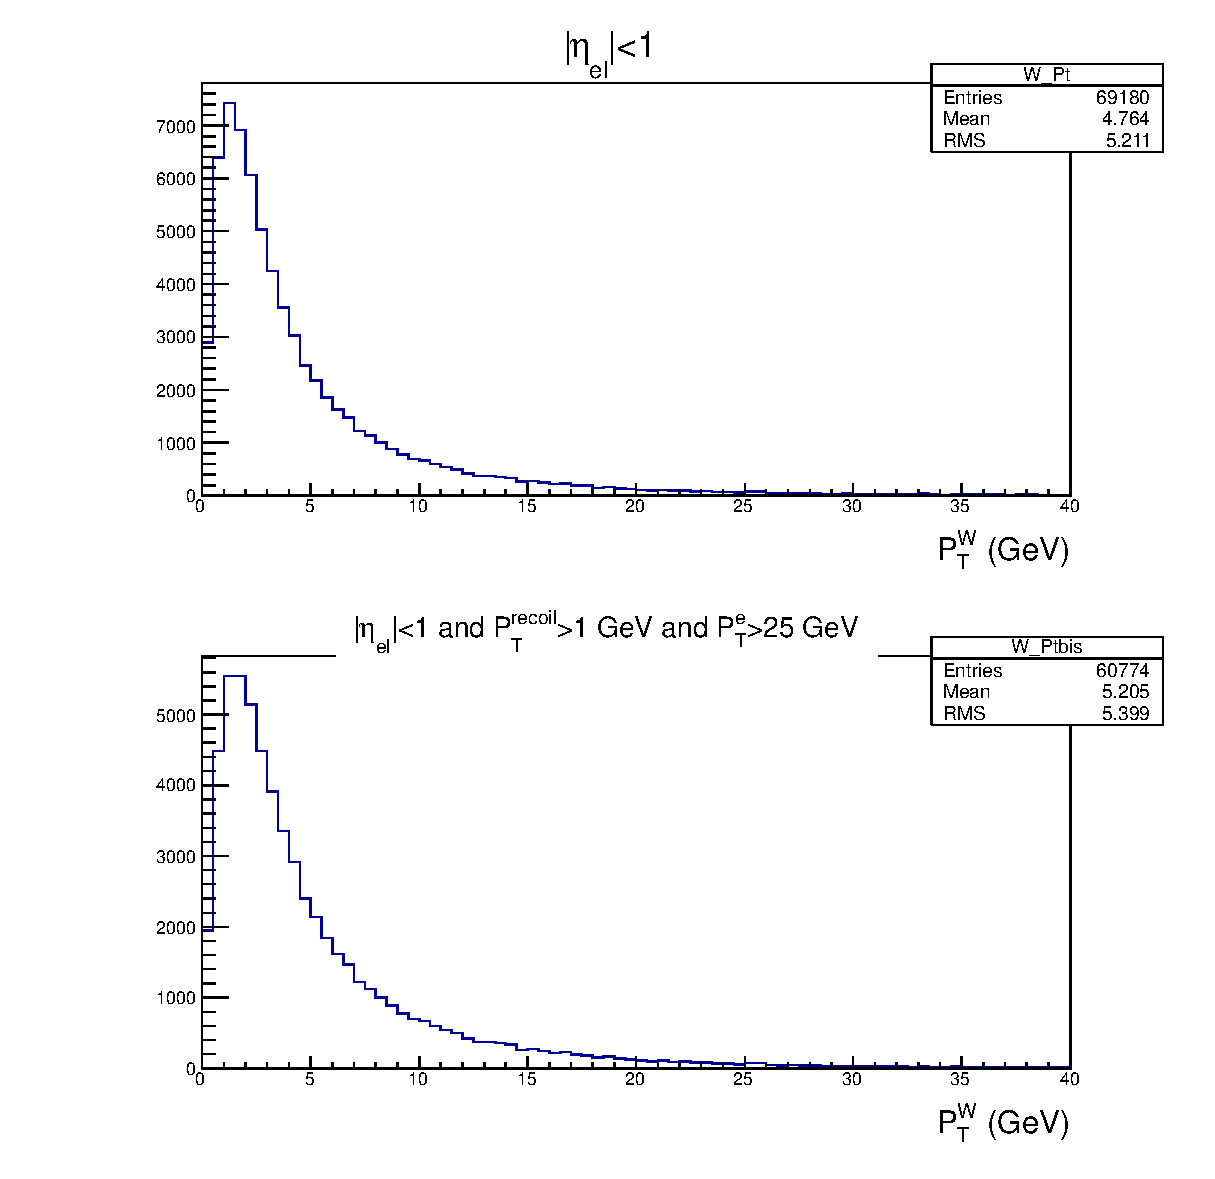
\includegraphics[width=10cm]{images/W_Pt.eps}
\end{center}
\caption{\label{fig:MC_W_Pt} Expected distribution of the transverse momentum of the produced W boson, $P^W_T$.}
\end{figure}

\begin{figure}[tbhp]
\begin{center}
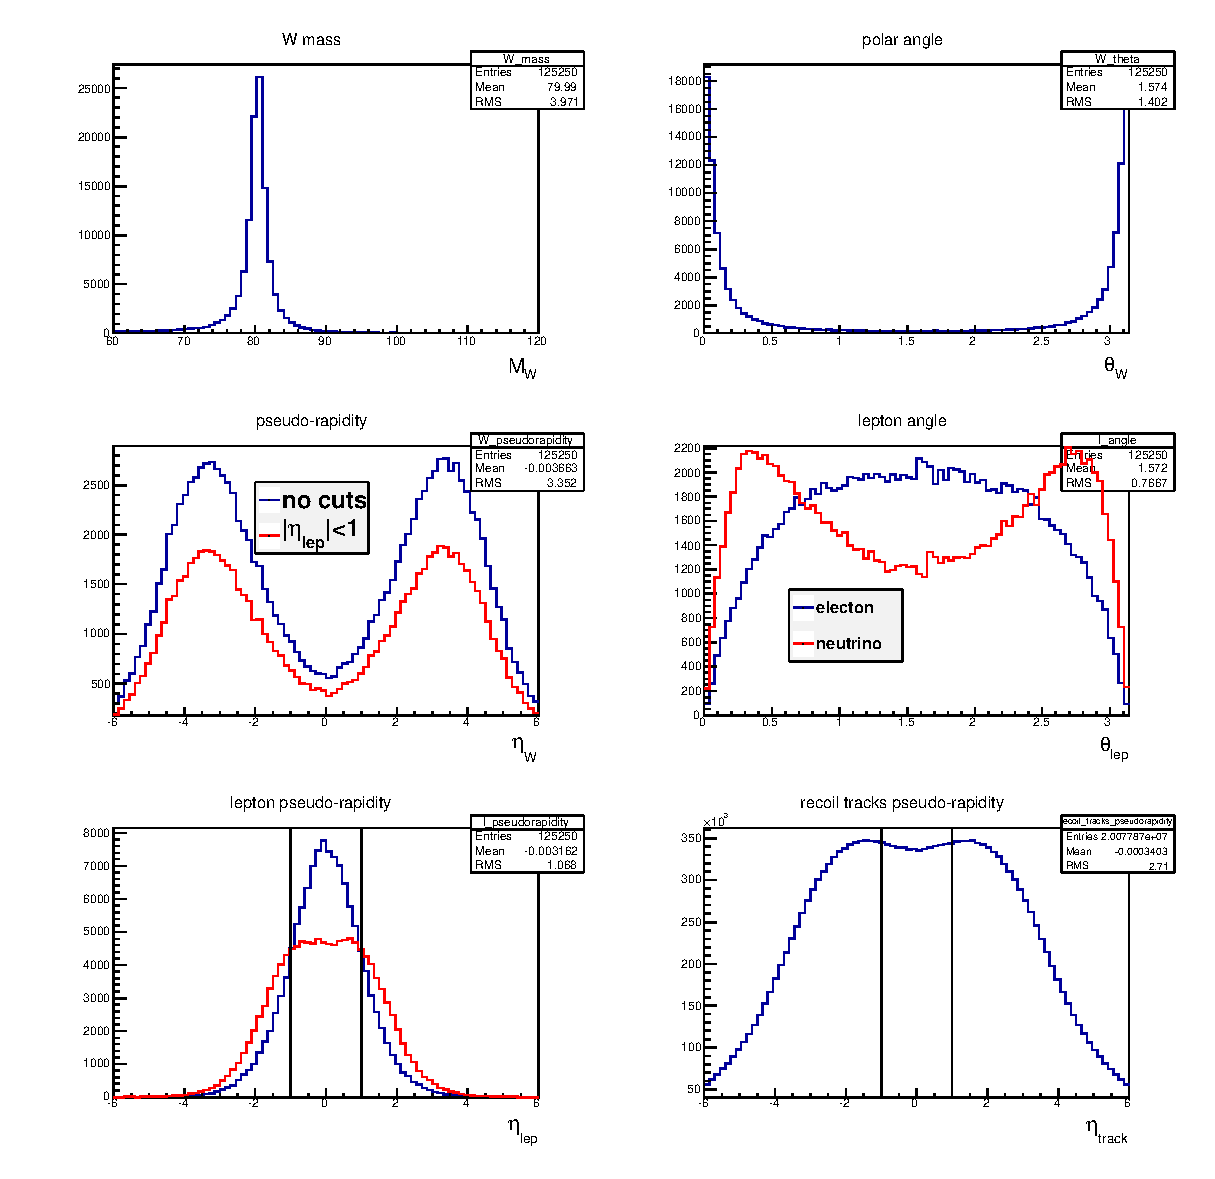
\includegraphics[width=14cm]{images/W_rapidity.eps}
\end{center}
\caption{\label{fig:MC_W_eta} W-mass; polar angles and pseudo rapidity distributions of the produced W, the decay leptons and the recoil tracks.}
\end{figure}

Most of the recoil tracks in the BARREL region are expected to carry a very
small fraction of the energy as shown in fig.~\ref{fig:MC_recoil_Efrac}.

\begin{figure}
\centering
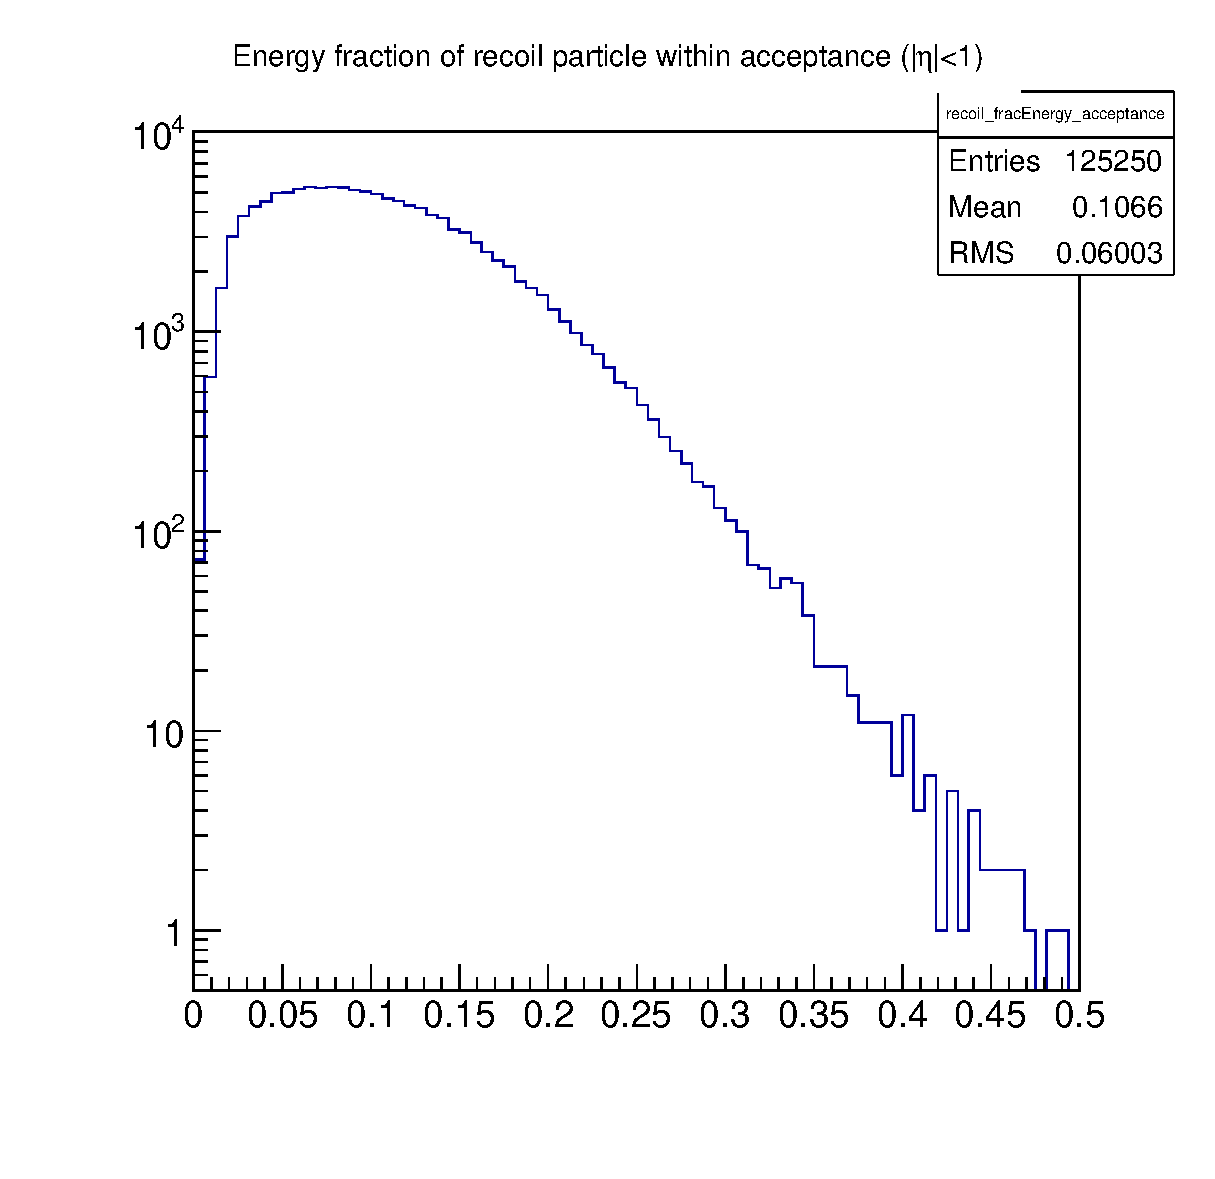
\includegraphics[height=0.5\textheight]{images/recoil_energy_frac.eps}
\caption{Expected fraction of energy carried by recoil particles within the BARREL region ($|\eta|<1$).}
\label{fig:MC_recoil_Efrac} 
\end{figure}

We can use MC to correct for the missing $P_{T}$ in the recoil tracks due to
the limited acceptance of the STAR detector. \textit{Such a procedure will
introduce a model-dependent systematic which will grow with the value of the
correction.}
%Nevertheless values of the corrections up to 30-40\% are considered acceptable...

We estimate the statistical power of the $A_N$ measurement for an integrated
luminosity of $300~\text{pb}^{-1}$. As a basis we use the total $W^\pm$ and
$Z^0$ yields observed at STAR in Run 9. The $W$ and $Z$ candidate events,
$N_\text{obs}$, along with the backgound numbers, $N_\text{bkg}$, are borrowed
from the earlier STAR analysis~\cite{WCrossSecRun9} that reported the production
cross section using $\approx 13~\text{pb}^{-1}$ of inegrated luminosity:
%
%$N_{W/Z} = N_\text{obs} - N_\text{bkg}$
%
\begin{align*}
N_{W^+} &= 496 - 37 = 459,\\
N_{W^-} &= 148 - 26 = 125,\\
N_Z &= 13 - 0 = 13.
\end{align*}
%
To reflect the expected increase in the integrated luminosity we scale the
above numbers a factor $\approx 23$. In order to illustrate the sensitivity of
the future measurement to the non-vanishing $W$ and $Z$ $A_N$ we calculate the
relative yields in bins of the boson rapidity from the MC sample. The expected
statistical power of $A_N$ in bins of $W$ rapidity is shown in
Figure~\ref{fig:MC_Wmeas_stat} for $W^+$ and $W^-$ respectively compared with
theoretical prediction from~\cite{Kang:2009bp}.

\begin{figure}
\subfloat[$W^+$]{\includegraphics[width=0.49\textwidth]{images/anapow_w_plus} \label{fig:MC_Wmeas_stat_plus} }
\subfloat[$W^-$]{\includegraphics[width=0.49\textwidth]{images/anapow_w_minus}\label{fig:MC_Wmeas_stat_minus}}

\caption[]{Expected statistical uncertainties for measured asymmetry $A_N$ of
$W^+$ \subref{fig:MC_Wmeas_stat_plus} and $W^-$ \subref{fig:MC_Wmeas_stat_minus}
decaying leptonically at STAR as a function of the boson's rapidity.}

\label{fig:MC_Wmeas_stat} 
\end{figure}


\newpage

\begin{thebibliography}{9}

\bibitem{WCrossSecRun9}
``Measurement of the W and Z Production Cross Sections at Mid-rapidity in Proton-Proton Collisions at $\sqrt{s} = 500$~GeV in Run~9,'' STAR~Note~0546.

%\cite{Kang:2009bp}
\bibitem{Kang:2009bp} 
  Z.~-B.~Kang and J.~-W.~Qiu,
  ``Testing the Time-Reversal Modified Universality of the Sivers Function,''
  Phys.\ Rev.\ Lett.\  {\bf 103}, 172001 (2009)
  [arXiv:0903.3629 [hep-ph]].
  %%CITATION = ARXIV:0903.3629;%%

\end{thebibliography}

\end{document}
